%\documentclass[a4paper,12pt]{article}
\documentclass[14pt]{extarticle}

\usepackage{cmap}		
\usepackage[utf8]{inputenc}			
\usepackage[english,russian]{babel}
\usepackage{framed}
\usepackage{hyperref}
\usepackage{amsmath}
\usepackage{graphicx}
\usepackage[colorinlistoftodos]{todonotes}
\usepackage{wrapfig}
\usepackage{lipsum}
\usepackage{listings}
\usepackage{color}
\usepackage{indentfirst}
%\usepackage{times}
\usepackage{textcomp}
\usepackage{indentfirst}
\textheight=24cm % высота текста
\textwidth=16,5cm % ширина текста
%\oddsidemargin=30 mm %отступ от левого края
\oddsidemargin=0pt % отступ от левого края
\parindent=1,25cm
\topmargin=-2cm % отступ от верхнего края
\definecolor{mygray}{rgb}{0.4,0.4,0.4}
\definecolor{mygreen}{rgb}{0,0.8,0.6}
\definecolor{myorange}{rgb}{1.0,0.4,0}


\usepackage{setspace}
\usepackage{lipsum}

% ADD THE FOLLOWING COUPLE LINES INTO YOUR PREAMBLE
\let\OLDthebibliography\thebibliography
\renewcommand\thebibliography[1]{
  \OLDthebibliography{#1}
  \setlength{\parskip}{0pt}
  \setlength{\itemsep}{0pt plus 0.3ex}
}

\lstdefinestyle{customc}{
  belowcaptionskip=1\baselineskip,
  breaklines=true,
  frame=L,
  xleftmargin=\parindent,
  language=C,
  showstringspaces=false,
  basicstyle=\footnotesize\ttfamily,
  keywordstyle=\bfseries\color{green!40!black},
  commentstyle=\itshape\color{purple!40!black},
  identifierstyle=\color{blue},
  stringstyle=\color{orange},
  numbers=left,
  numbersep=13pt,
  numberstyle=\small\color{mygray},
}
\lstset{escapechar=@,style=customc}
\linespread{1.5}
\newcommand{\HRule}{\rule{\linewidth}{0.5mm}}

\begin{document}

%\begin{titlepage}
\begin{center}

\textsc{\Large Московский Физико-Технический Институт}\\
\textsc{\large (Национальный Исследовательский Университет)}\\[1.5cm]

% Upper part of the page. The '~' is needed because \\
% only works if a paragraph has started.

\includegraphics[width=0.25\textwidth]{img/logo.png}~\\[1cm]

\textsc{\Large Бакалаврская работа}\\[0.5cm]

% Title
\HRule \\[0.4cm]
{ \LARGE \bfseries Влияние вышестоящих регуляторных регионов и промоторов на связь между бактериофагами и их хозяевами \\[0.4cm] }

\HRule \\[1.5cm]

% Author and supervisor
\noindent
\begin{minipage}{0.4\textwidth}
\begin{flushleft} \large
\emph{Студент:}\\
Шарафутдинов Эмиль
\end{flushleft}
\end{minipage}%
\begin{minipage}{0.4\textwidth}
\begin{flushright} \large
\emph{Преподаватель:} \\
 Родригес Валера Франсиско Эдуардо
\end{flushright}
\end{minipage}

\vfill

% Bottom of the page
{\large 24 апреля 2021 г.}

\end{center}
\end{titlepage}


\begin{center}
\item \section{Аннотация}
\end{center}

\par{Бактериофаги (фаги) - это вирусы, которые избирательно поражают бактериальные клетки. Такая специфика обусловлена
зависимостью фага от клеточного механизма хозяина, который нужен фагу для репликации и синтеза вирусных компонентов.
Пример такой зависимости можно наблюдать у фага Т4 и E.coli \cite{hinton} или цианобактерии с её фагом 
\cite{puxty-evanx}.}

\par{В этой работе мы предположили, что такого рода зависимость между фагом и бактерией-хозяином можно 
наблюдать на генетическом уровне. Поскольку во многих известных случаях атаки фагами бактерий начинаются с захвата 
РНК-полимеразы бактерии, мы искали общие мотивы на промоторных областях у фагов и бактерий.}

\par{ В результате мы получили, что почти в половине случаев общие мотивы в этих областях у фагов и хозяинов есть. Также
в большинстве случаев мы нашли общие мотивы между различными фагами, атакующими одних и тех же бактерий. Таким образом, 
при поиске наличия взаимодействий между фагом и бактерией мы предлагаем поиск общих мотивов в промоторных областях фага 
и бактерии.}


\newpage
\begin{spacing}{1.2}
  \tableofcontents
\end{spacing}

\newpage
\begin{center}
\item \section{Введение}
\end{center}

    \begin{center}
    \item \subsection{Бактериофаги}
    \end{center}
    
    \begin{figure}[h]
        \centering
            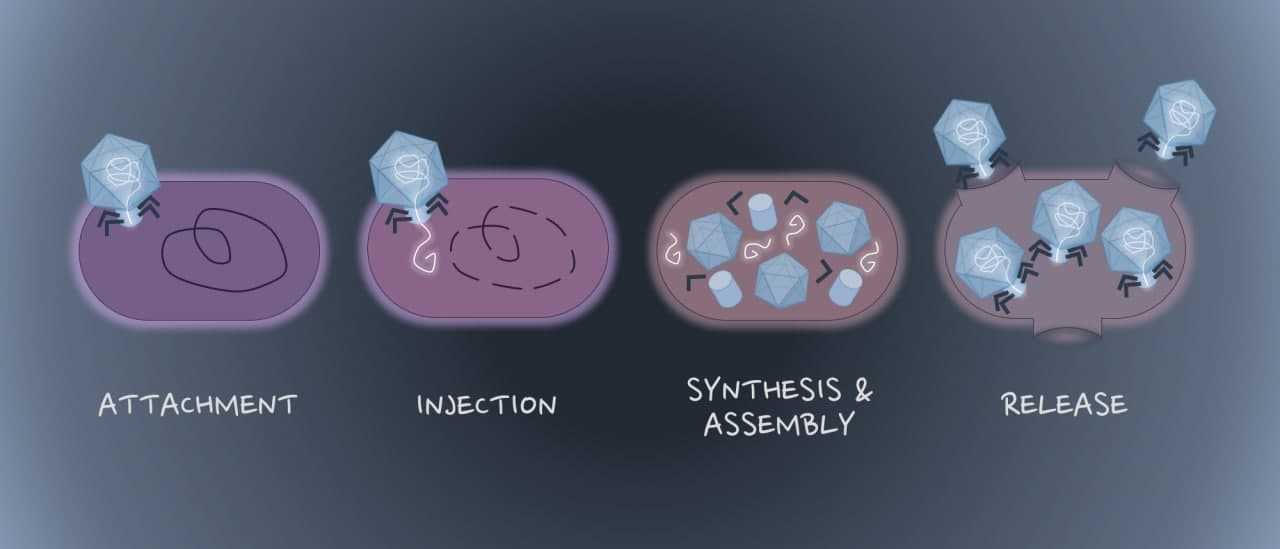
\includegraphics[width=\textwidth]{img/average_phage.jpg}
        \caption{Как фаг убивает бактерию. (1) Фаг сначала приземляется на бактерии. (2) Затем он вводит свою ДНК внутрь
        бактерий. (3) ДНК копируется и используется для изготовления капсидов для новых фагов. (4) Новые фаги собираются
        и взрывают бактерию, убивая её в процессе. \cite{advdisphage}}
        \label{fig:skybox}
    \end{figure}
    
	\par{Бактериофаги - это вирусы, которые заражают и размножается внутри бактерий и архей. Как правило, бактериофаги 
	состоят из белковой оболочки и генетического материала одноцепочечной или двуцепочечной нуклеиновой кислоты (ДНК 
	или, реже, РНК). Фаги размножаются внутри бактерии после введения своего генома в ее цитоплазму. 
	\cite{phagewikieng}}
	
	\par{Более 90\% бактериофагов имеют большие геномы в виде двухцепочечных ДНК. Они относятся к трем основным 
	морфологическим группам бактериофагов: Myoviridae (с длинными, жесткими, сократительными хвостами), Siphoviridae
	(с длинными, гибкими, неконтрактирующими хвостами) и Podoviridae (с короткими, неконтрактирующими хвостами). 
	\cite{phageapps}}
	
	\par{Для бактерии исход заражения бактериофагом может быть разным. Некоторые бактериофаги вызывают лизис и гибель 
	клетки в течение очень короткого времени. Как правило, это приводит к рождению сотен новых вирусов в течение 
	нескольких минут или часов. Это процесс, который может повторяться до тех пор, пока их бактерии 
	присутствуют в достаточном количестве для поддержки репликации. Многие бактериофаги ведут себя именно так (иногда их
	называют вирулентными) и не способны продуцировать какой-либо другой вид инфекции. Есть также умеренные 
	бактериофаги, которые заражают клетки, а затем становятся спящими в латентном состоянии: реплицируются вместе с 
	хромосомой хозяина и впоследствии передаются каждой дочерней клетке после деления. Однако эти дремлющие фаги могут 
	быть активированы несколько причинами, например повреждением ДНК. Для некоторых бактериофагов хромосомная ДНК 
	хозяина может быть упакована в частицы бактериофага во время репликации бактериофага вместо генома бактериофага. Это
	может привести к высокому уровню горизонтального переноса генов в бактериальной популяции.  \cite{phagetreat}}
    
    \begin{center}
    \item \subsubsection{Использование бактериофагов}
    \end{center}
    
    \par{Использование бактериофагов в качестве высокоспецифичных антимикробных средств широко документировано в 
    литературе. Их даже можно использовать в качестве регулируемого терапевтического средства.}
    
    \par{Как уже было сказано, в большинстве случаев, бактериофаги не дают бактерии размножаться, а вместо этого она 
    производит дополнительные фаги. В то время, когда по каким-либо причинам химические антибиотики 
    могут не сработать, фаги могут быть хорошей заменой для них \cite{phageapps}. Преимущества включают снижение 
    побочных эффектов и снижение риска развития резистентности бактерии. Недостатки включают трудность поиска 
    эффективного фага для конкретной инфекции. \cite{advdisphage}}
    
    \par{Фаги применяются не только в медицине. Они могут использоваться в пищевой промышленности, их 
    используют в качестве противодействия биологическому оружию и токсинам, в диагностике (например, для поиска 
    стафилококка в крови), в молочной промышленности. У фагов также широко используются в разных биологических 
    исследованиях \cite{phagewikieng}}
    
    \begin{center}
    \item \subsubsection{Мотивы}
    \end{center}
    
    \par{Мотив последовательности ДНК, РНК или белка - это короткий паттерн, который сохраняется во время эволюции. 
    Мотивом в ДНК может может быть сайт связывания белка; в белках мотив может быть активным сайтом фермента или 
    структурной единицей, необходимой для правильного сворачивания белка. Мотивы в последовательностях являются одними 
    из основных функциональных единиц молекулярной эволюции.}
    
    \par{Многие геномы фагов кодируют небольшие белки, которые специфически изменяют РНК-полимеразу (RNAP)
    бактериального хозяина, ингибируя транскрипцию бактериальной ДНК и способствуя регулируемой транскрипции фаговой 
    ДНК.}    
    
    \par{Транскрипция бактерии начинается со связывания $\sigma$-фактора с каталитическим ``ядром'' RNAP. Начальный 
    $\sigma$-фактор, $\sigma^{70}$, специфично связывается с отдельными нуклеотидными последовательностями(мотивами) в 
    промоторе. Я описываю этот процесс для E.coli детальнее ниже. Фаги развили механизмы, которые модифицируют 
    $\sigma^{70}$ и перенаправляют бактериальную RNAP для транскрипции генов фага.}
    
\newpage
\begin{center}
\item \section{Цель и задачи} \label{sec:code}
\end{center}

    \par{Как было показано, фаги имеют широкое применение в самых разных областях. Понимание устройства фагов в природе 
    и принципов их работы может упростить и/или улучшить способы их использования. В этой работе улучшить понимание 
    взаимодействия между бактериофагами и бактериями. Мы хотим обнаружить общие мотивы 
    у фагов и бактерий, которых они атакуют, в промоторных участках их последовательностей ДНК.}
    
    \par{Также нам интересно исследовать наличие общих мотивов в промоторных последовательностях между фагами. Мы хотим 
    проверить, является ли наличие общих мотивов в промоторных областях фагов свидетельством их родства или близости.}

\newpage
\begin{center}
\item \section{Обзор литературы} \label{sec:math}
\item \subsection{Взаимодействие фага Т4 и E.coli}
\end{center}
        
        \par{Экспрессия генома Т4 - это строго регулируемый процесс, который начинается сразу после заражения хозяина. 
        Основной контроль над этой экспрессией происходит на уровне транскрипции. Т4 не кодирует свою собственную 
        РНК-полимеразу (RNAP), а вместо этого кодирует множество факторов, которые служат для изменения специфичности 
        полимеразы хозяина по мере развития инфекции. Изменения полимеразы хозяина сопровождаются с тремя классами 
        транскрипции фага: ранней, промежуточной и поздней. Ранняя и промежуточная РНК (РНК, образовавшаяся при ранней и
        промежуточной транскрипции) обнаруживается дорепликативно 
        \cite{hinton1,hinton2,hinton3,hinton4,hinton5,hinton6}, в то время как поздняя транскрипция сопровождается 
        репликацией Т4 и нам в нашей работе не интересна. Ранние транскрипты T4 генерируются из ранних промоторов 
        (Pe),которые активны сразу после инфицирования. Промежуточные транскрипты Т4 генерируются примерно через 1 
        минуту после заражения при \(37^\circ C\) и требуют синтеза белка фага. Средняя РНК синтезируется двумя 
        способами: 1) активация промежуточных промоторов (Pm) и 2) расширение транскриптов Pe из ранних генов в 
        нижестоящие средние гены.}
        
        \begin{center}
        \item \subsubsection {Начало транскрипции E.coli}
        \end{center}
        
        \par{E. coli RNAP холофермент, как и все бактериальные RNAP, состоит из ядра субъединиц 
        \((\beta,\beta',\alpha_1,\alpha_2\) и \(\omega)\), которое содержит активный сайт для синтеза РНК, и фактора 
        специфичности \(\sigma\), который распознает промоторы в ДНК и устанавливается на начальный сайт для 
        транскрипции. Первичный \(\sigma\), \(\sigma^{70}\) в E. coli, используется во время экспоненциального роста; 
        альтернативные факторы \(\sigma\) направляют транскрипцию генов, необходимых в различных условиях роста или во 
        время стресса \cite{17}}
        
        \par{Для начала транскрипции части RNAP должны сначала распознать и связаться с двухцепочечными (ds) элементами 
        распознавания ДНК, присутствующими в промоторе \cite{20}. Каждый из C-концевых доменов 
        $\alpha$-субъединиц ($\alpha$-CTDS) может взаимодействовать с вышестоящим элементом, A/T богатыми 
        последовательностями, присутствующими между позициями -40 и -60. Части \(\sigma^{70}\), присутствующие в RNAP, 
        могут взаимодействовать с тремя различными элементами dsDNA: с элементом -35, с последовательностью -15TGn-13 
        (TGn) и с позициями -12/-11 элемента -10. Как правило, промотор должен содержать только два из трех 
        \(\sigma^{70}\)-зависимых элементов для активности; таким образом, промоторы E. coli могут быть свободно 
        классифицированы как -35/-10 (основной класс), TGn/-10 (также называемый расширенным -10) или -35/TGn 
        \cite{20}.}
        
        \begin{center}
            \item \subsubsection{Этапы транскрипции фага Т4}
        \end{center}
        
        \begin{figure}[h]
            \centering
                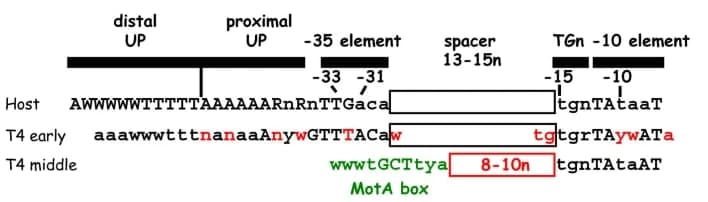
\includegraphics[width=\textwidth]{img/Hinton.jpg}
            \caption{\textit{Сравнение последовательностей хоста E. coli, раннего Т4 и промежуточного промоторов Т4.}
            Сверху показаны последовательности и положения элементов распознавания промотора хозяина для
            $\sigma^{70}$-RNAP (UP, -35, TGn, -10)\cite{20}. Ниже аналогичные последовательности, обнаруженные в 
            ранних \cite{4} и промежуточных \cite{91} промоторах T4, сходства выделены черным цветом, а 
            различия-красным. W = A или T; R = A или G; Y = C или T, n = любой нуклеотид; заглавная буква представляет 
            собой более высоко консервативное основание. \cite{hinton}}
            \label{fig:skybox}
        \end{figure}

        \par{Т4 заражает E.coli только во время экспоненциального роста. Транскрипция ранних генов Т4 начинается сразу 
        после заражения. Таким образом, для эффективной инфекции фаг должен быстро перенаправить 
        \(\sigma^{70}\)-ассоциированный RNAP, который активно участвует в транскрипции генома хозяина, на ранние 
        промоторы T4. Такое немедленное перенаправление часто происходит успешно отчасти потому, что большинство ранних 
        промоторов T4 содержат такие же элементы распознавания \(\sigma^{70}\)-RNAP (-35, TGn и -10 элементов) и 
        элементы \(\alpha\)-CTD UP (списки известных последовательностей ранних промоторов T4 в \cite{4}). Тем не
        менее, выравнивание последовательностей ранних промоторов Т4 показало дополнительные области совпадения, и есть 
        предположение, что они содержат и другие последовательности, которые могут оптимизировать взаимодействие RNAP 
        хозяина с элементами промотора T4. Следовательно, в отличие от большинства промоторов хозяина, которые относятся
        к классам -35/-10, TGn/-10 или -35/TGn, ранние промоторы T4 могут быть описаны как ``супер'' UP/-35/TGn/-10 
        промоторы \cite{hinton}. Действительно, большинство ранних промоторов Т4 очень хорошо конкурируют с промоторами 
        хозяина за доступный RNAP \cite{39}.}
        
\begin{center}
    \item \subsection{Взаимодействие цианофага и цианобактерии}
\end{center}
    
    \par{В этой статье авторы инетересовались изменением климата. Изучение этого вопроса требуте детального знания о
    биологической трансформации углерода на Земле. Стало очевидно, что океан - это важный поглотитель
    атмосферного углекислого газа. В плане поглощения $CO_2$ в открытом океане доминируют доминируют два организма: 
    Prochlorococcus и Synechococcus \cite{3_,4_}. Эти организмы стали моделью для изучения потока углерода из $CO_2$ 
    в микробную жизнь \cite{5_,6_}. Однако биологическик потери (антагонистические взаимодействия, выпас скота, вирусный
    лизис) прохлорококка и синехокка мало изученны. У вирусов только открывают новые гены, которые действовуют для 
    поддержания фотосинтеза во время инфекции \cite{8_}, так что, несмотря на окончательную потерю фиксированного 
    углерода в растворенном органическом веществе в результате лизиса, фиксация $CO_2$ может поддерживаться временно в 
    течение относительно длительных латентных периодов вируса. Недавно было показано, что на самом деле цианофаг 
    отключает $CO_2$ инфекцию на ранних стадиях заражения, но при этом поддерживает реакции фотосинтеза \cite{9_}.}
    
    \begin{center}
        \item \subsubsection{Влияние интенсивности света на транскрипцию фага}
    \end{center}


    \begin{figure}[]
            \centering
            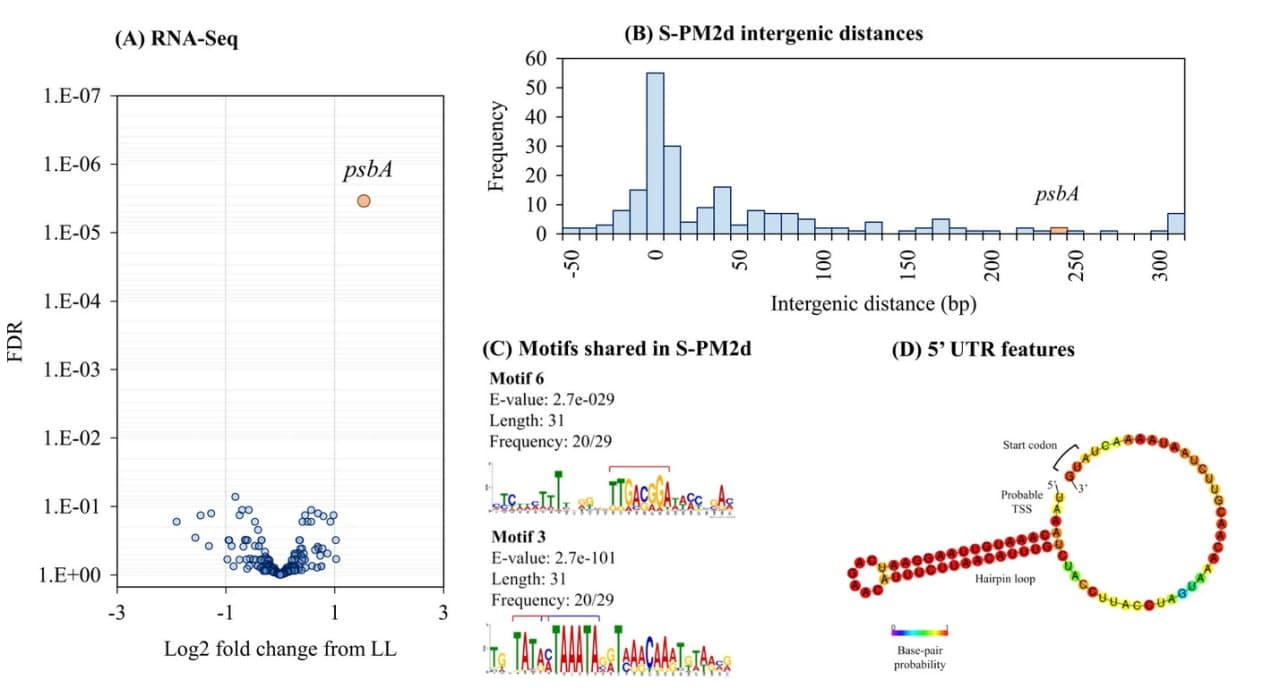
\includegraphics[width=\textwidth]{img/protein.jpg}
            \caption{\textit{Влияние интенсивности света на глобальную экспрессию генов.} \textbf{a} Вулкано-плот с
            логарифмической шкалой, показывающий относительное изменение транскриптом (относительно воздействия слабого
            света). Ось y показывает скорректированное p-значение ложного обнаружения, рассчитанное с помощью edgeR.
            Оранжевый круг показывает статистически значимую дифференциальную экспрессию генов по edgeR. \textbf{b}
            Гистограмма длин вышестоящих межгенных последовательностей в геноме цианофага S-PM2d. Ячейка, содержащая
            psbA, показана оранжевым цветом. \textbf{c} Мотивы вышестоящих последовательностей ДНК, обнаруженных у
            цианофаговых PSBA. Красные полосы указывают на -35 и -10 элементы сайтов связывания $\sigma^{70}$, а синяя
            полоса показывает сайт связывания для $\sigma$ Gp55. \textbf{d} Предсказываемая структура складывания петли
            шпильки S-PM2d psbA 5'-UTR \cite{puxty-evanx}}
            \label{fig:skybox}
    \end{figure}
    
    \par{Авторы обнаружили что скорость транскрипции фагов при сильном свете увеличивается, в то время, как репликации
    ДНК была такой же, как и при слабом. Авторы обнаружили, что скорость экспрессии только одного гена цианофага была
    пропорциональна интенсивности света. Это был фотосинтетический AMG psbA, кодирующий полипептид D1, расположенный в
    ядре центра реакции PSII. Synechococcus также кодируют это белок, но у них не было никаких увеличений в скорости 
    транскрипции. \cite{puxty-evanx}}
    
    \par{Цианобактерии, включая морской Synechococcus, демонстрируют светозависимую транскрипцию psbAs \cite{18_,23_}. В
    модельной цианобактерии на светозависимое изменение транскриптов psbA влияют несколько факторов, включая 
    альтернативные $\sigma$-факторы \cite{24_,25_}. Более того, продукты деградации D1 непосредственно связываются с 
    вышележащими регионами последовательностей psbA, так что вызванное светом повреждение может положительно влиять на 
    транскрипцию psbA. Авторы не смогли найти консервативные мотивы в вышележащих областях в последовательностях psbA 
    S-PM2d, которые были бы общими с Synechococcus.} 
    
    \par{Межгенную вышестоящая регуляторная последовательность у psbA нехарактерно длинная у S-PM2d(232 пар 
    нуклеотидов,по сравнению с медианой 6 по всему геному). Это также справедливо и для других цианофагов, где 
    вышестоящие регуляторные области psbA варьируют в пределах 125-453 пн. Также с высокой степенью достоверности  было 
    обнаружено между рассмотренными фагами 6 общих мотивов в этих последовательностях \cite{puxty-evanx}. Из них два 
    присутствовали в S-PM2d. Эти два мотива - это  -35 (мотив 6) и -10 (мотив 3) (на рисунке) элементы сайтов связывания
    фактора транскрипции $\sigma^{70}$, типичные для ранних генов Т4-подобных фагов \cite{31_}. К тому же, было 
    обнаружено, что как и у T4, мотив 3 содержит сайт для посадки позднего $\sigma$-фактора Gp55. Таким образом, у 
    S-PM2d имеются мотивы, необходимые для скоординированной экспрессии psbA на начальной и поздней стадиях инфекции.}
    
    \begin{center}
        \item \subsection{GeneMarkS-2}
    \end{center}
    
    \par{Для поиска прокариотических генов существует несколько инструментов (например GeneMarkS, Glimmer3, Prodigal), 
    которые известны достаточно высокой точностью в предсказании белок-кодирующих ORF. В среднем эти инструменты 
    способны найти более 97\% генов в проверенном тестовом наборе с точки зрения правильного предсказания концов гена 3'
    \cite{hyatt}. Кроме того, точность определения стартов генов 
    составляет в среднем 90\% \cite{hyatt}. Но основная часть генов, которые не были обнаружены, принадлежали в 
    основном к атипичной категории, т. е. гены с паттернами, не соответствующими видоспецифической натренированной 
    модели, обученной на основной части генома \cite{bordov1}. Тем не менее авторы описали метод, с помощью 
    которого можно получить более высокую точность в обнаружении генов. \cite{lomsad}}
    
    \begin{figure}[]
            \centering
            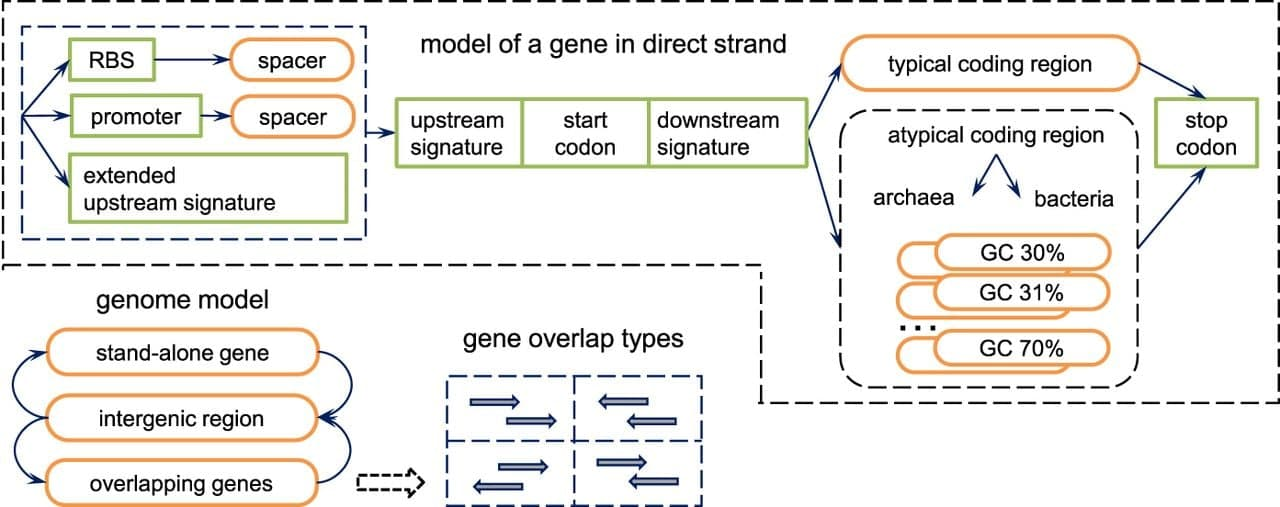
\includegraphics[width=\textwidth]{img/gms2_1.jpg}
            \caption{Диаграмма основного состояния обобщенной скрытой марковской модели (GHHM) геномной 
            последовательности прокариот. Состояния, показанные на верхней панели, использовались для моделирования гена
            в прямом направлении. Гены в обратном направлении моделировались идентичным набором состояний (с обратными 
            направлениями перехода). Различные состояния, моделирующие гены в прямых и обратных цепочках, были связаны 
            через состояние межгенной области или же перекрывающимися участками в противоположных цепочках. 
            \cite{lomsad}}
            \label{fig:skybox}
    \end{figure}
    
    \par{GeneMarkS-2 использует довольно сложную модель гена (рис. 4). Большинство белок-кодирующих областей в 
    прокариотических геномах имеют видоспецифичные паттерны из нескольких олигонуклеотидов (например, кодонов)
    \cite{fickett}. GeneMarkS-2 изучает эти паттерны и оценивает параметры типичной модели белок-кодирующих областей, 
    трехпериодической цепи Маркова \cite{bordov2}, итеративно самообученаясь на всем геноме.}
    
    
    \par{Алгоритм обучения без учителя выполняет несколько двухэтапных итераций (рис. 5). Каждая итерация приводит к (1)
    сегментации генома на кодирующие белки (CDS) и некодирующие области (прогнозирование генов) и (2) переоценке 
    параметров модели.}
    
    \begin{figure}[]
            \centering
            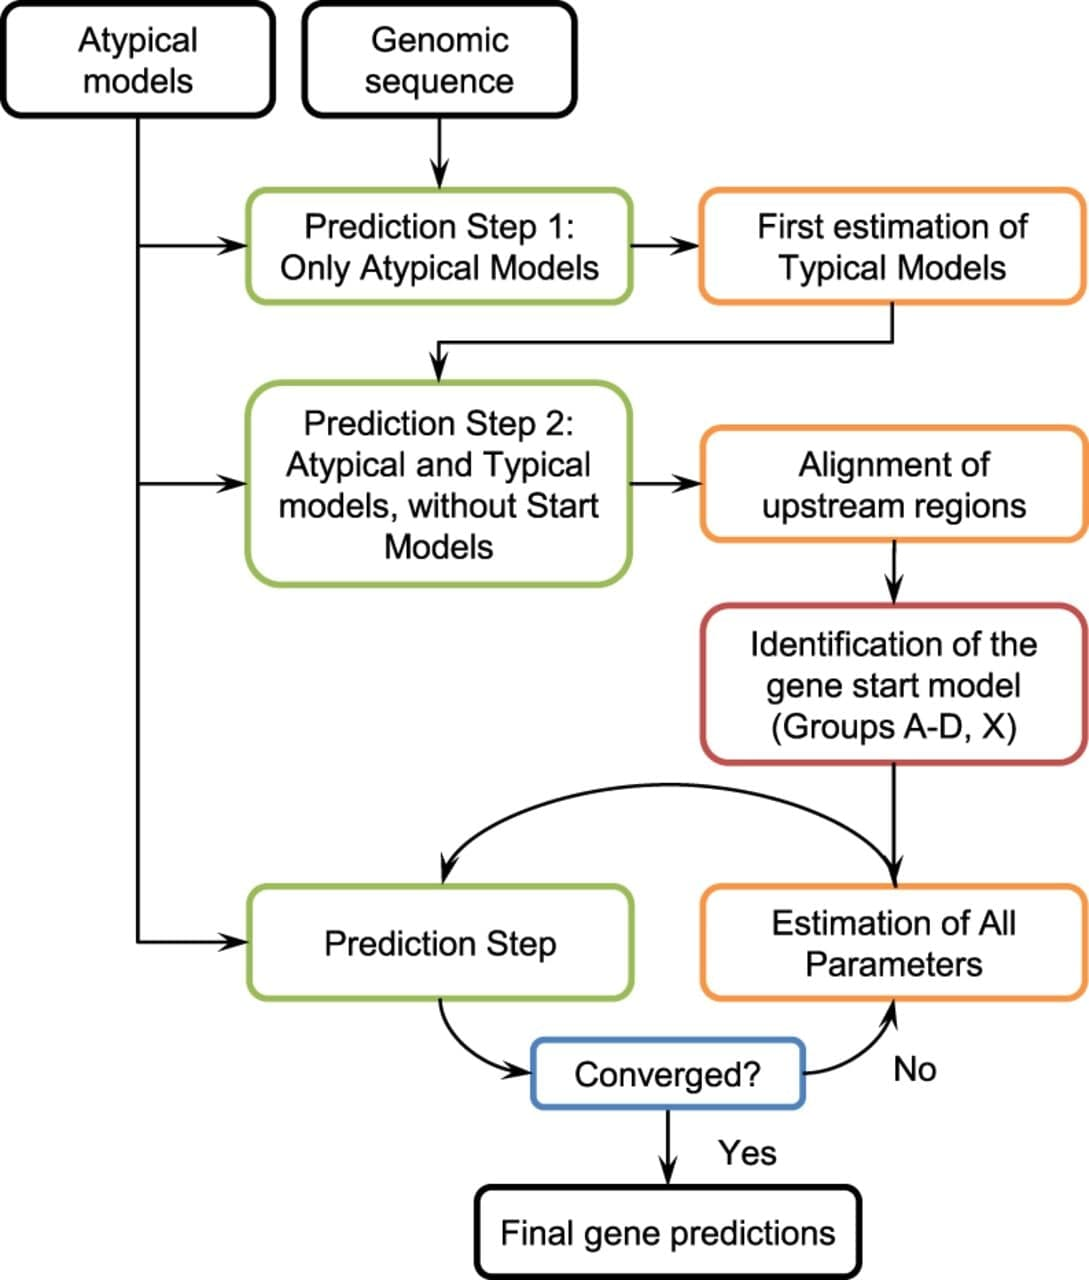
\includegraphics[width=\textwidth]{img/gms2_2.jpg}
            \caption{Диаграма обучения без учителя для GMS-2 \cite{lomsad}}
            \label{fig:skybox}
    \end{figure}
    
    
    \par{\textit{На первой итерации} Алгоритм Витерби вычисляет максимально вероятную 
    последовательность скрытых состояний (рис. 4) вдоль генома. После первого запуска
    алгоритма Витерби все участки генома, помеченные как ``белок-кодирующие'', собираются в обучающий набор для оценки 
    параметров ``типичной'' (для данного генома) модели. Аналогично помеченные как ``некодирующие'' участки нужны для 
    оценки параметров модели некодирования, которая строется в виде однородной цепи Маркова второго порядка.}
    
    
    \par{\textit{На второй итерации} Модель уже выбирает последовательности, расположенные вокруг запусков генов, 
    и выводит модели паттернов, кодирующих регуляцию транскрипции и/или трансляции. \textit{Третью итерацию и 
    далее} GeneMarkS-2 продолжает шаги предсказаний/оценок до тех пор, пока не 
    будет выполнено условие сходимости (99\% идентичности в гене начинается между последовательными итерациями).}
    
    
    \par{Для нас было важно, что наблюдаемая частота ошибок GeneMarkS-2 составила 4,4\%, за ней последовали Prodigal на 
    уровне 6,1\%, GeneMarkS на уровне 10,2\% и, наконец, Glimmer3 на уровне 13,2\%. Таким образом, GeneMarkS-2 сделал 
    наибольшее количество правильных прогнозов среди четырех искателей генов. \cite{lomsad}}
    
    \begin{center}
        \item \subsection{The MEME-Suite}
    \end{center}
    
    \par{The MEME-Suite - это программируемый набор инструментов, которые анализируют мотивы последовательностей. Ядром 
    набора является алгоритм обнаружения мотивов \texttt{MEME}, который находит мотивы в невыравненных 
    последовательностях ДНК, РНК или белков \cite{_1}. Поисковик мотивов ищет \textit{новые} мотивы в предоставленных 
    последовательностях. Существует много инструментов, предназначенных для поиска мотивов только в ДНК; The MEME-Suite 
    может искать мотивы и сканирование последовательностей ДНК, РНК и белков. \cite{bailey}}
    
    \begin{figure}[]
        \centering
        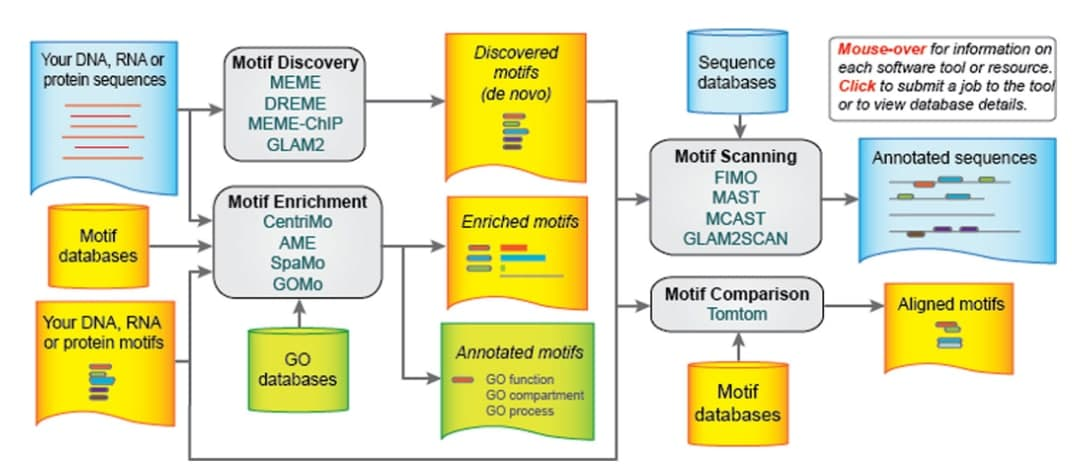
\includegraphics[width=\textwidth]{img/meme.jpg}
        \caption{Что умеет делать The MEME-Suite. Нам нужно находить новые мотивы в последовательностях - это 
        указано сверху посередине. \cite{bailey}}
        \label{fig:skybox}
    \end{figure}
    
    \par{Как было описано выше, алгоритм \texttt{MEME}, обнаруживает один или несколько мотивов в наборе 
    последовательностей ДНК, РНК или белков, используя метод максимизации математического ожидания для подгонки 
    двухкомпонентной конечной модели к набору последовательностей. Путём подгонки модели к данным обнаруживается 
    единичный мотив, дальше модель стирает вхождения максимально вероятного мотива, найденного таким образом и процесс 
    повторяется. Таким образом ищется множество мотивов. У алгоритм два необходимых параметра - минимальная и 
    максимальная ширина искомых мотивов. Он возвращает профиль каждого мотива и порог, которые вместе могут быть 
    использованы в качестве байесовского оптимального классификатора для поиска вхождений мотива в других базах данных. 
    Алгоритм оценивает, сколько раз каждый мотив встречается в каждой последовательности в наборе данных, и выводит 
    частоту встречаемости этого мотива. \cite{meme}}
    
    
\newpage
\begin{center}
\item \section{Методы} \label{sec:code}
\item \subsection{Программные средства}
\end{center}
\begin{itemize}
    \item Virus-Host DB - База данных Virus-Host организует данные о взаимоотношениях между вирусами и их хостами,
    представленные в виде пар идентификаторов таксономии NCBI для вирусов и их хостов. \cite{virus-host}
    
    \item GeneMarkS-2 - программное обеспечение для поиска генов внутри геномов. \cite{lomsad}
    
    \item NCBI Entrez Programming Utilities - программное обеспечение, набор из восьми серверных программ, которые
    обеспечивают стабильный интерфейс с системой запросов и баз данных Entrez в Национальном центре биотехнологической
    информации (NCBI) \cite{entrez}
    
    \item Biopython - набор инструментов для биологических вычислений, написанных на Python. \cite{biopython}
    
    \item The MEME Suite - программное обеспечение для поиска новых, нераскрытых мотивов (повторяющихся паттернов
    фиксированной длины) в последовательностях. МЕМ разбивает паттерны переменной длины на два или более отдельных
    мотива. \cite{bailey}
    
    \item Python 3.8.5 - среда для запуска скриптов формата *.py \cite{python}
    
    \item Jupyter Notebook -веб-приложение, которое позволяет создавать и обмениваться
    документами, содержащими живой код, уравнения, визуализации и повествовательный текст.\cite{jupyter}
    
    \item Скрипты отсюда \(https://github.com/poolsar42/phages-and-hosts\) - подумать, что про них написать!
    \cite{github}
    
    \item \(Fasta\_merge.ipynb\) - скрипт для объединения регуляторных областей хозяина и его фагов в один файл.
    \item \(Hosts\_upstream\_regions.ipynb\) - скрипт для выделения регуляторных областей.
    \item \(Proteins\_formation.ipynb\) - скрипт для сбора белковых последовтельностей в один файл.
    \item \(Searching\_host\_genomes.ipynb\) - скрипт для выгрузки необходимых к работе геномов хостов.
    \item \(Unpacking.ipynb\) - скрипт для распаковки выгруженных геномов.
    \item \(VH\_tsv\_writer.ipynb\) - скрипт, выписывающий в файл ID хоста и ID прилежащих к нему фагов.
    \item \(Virus\_genes.ipynb\) - скрипт для выгрузки геномов фагов.
    \item \(missing\_phage\_genomes.ipynb\) - скрипт для поиска фагов, для которых GMS2 не находит гены.
    \item \(proteins\_convertation.ipynb \) - скрипт для преобразования \\ ДНК-последовательностей
                                в белковые.
    \item \(regex\_promoter.ipynb \) - скрипт для анализа полученных результатов
    \item \(run\_gms2.py\) - скрипт для поиска генов в геномах с помощью GeneMarkS-2
    \item \(tsv\_write.ipynb\) - скрипт для выписывания информации о связи между хостами и фагами в один файл
\end{itemize}

\begin{center}
      \item \subsection{Получение общих мотивов}
      \item  \subsubsection{Выгрузка геномов}
\end{center}
    \begin{itemize}
        \item С FTP сервера Virus-Hist DataBase выгрузили файл virushostdb.tsv - в нём содержится информация о связи 
        между фагами и их хостами.
        \item С помощью \(tsv\_write.ipynb\) - выписали в удобном формате все взаимоотношения между фагами и 
        хостами.
        \item С помощью \(Virus\_genes.ipynb\) - выгрузили геномы фагов.
        \item Запустили \(Searching\_host\_genomes.ipynb\) - для выгразки геномов хостов.
        \item И распаковали с помощью \(Unpacking.ipynb\).
    \end{itemize}
    
    \par{Мы собрали геномы всех фагов, которые находятся в базе данных Virus-Host DB, там для каждого фага также был 
    указан или были указаны хосты, к которым он может прикрепиться. Их RefSeq ID. Мы всё выгрузили с FTP сервера. Геномы
    хостов затем выгрузили с базы данных RefSeq NCBI}

    \begin{center}
    \item \subsubsection{Получение вышестоящих регуляторных регионов}
    \end{center}
        \begin{itemize}
            \item Запустили скрипт \(run\_gms2.py\) ждя поиска генов во всех имеющихся геномах
            \item И далее запустили \(Hosts\_upstream\_regions.ipynb\) для выделениях областей длиной 50 нуклеотидов 
            перед точкой начала транскрипции у каждого найденным геном
        \end{itemize}
    \par{Гены мы находили с помощью Gene-Marks 2. Gene-Marks 2 также дал позицию каждого гена в геноме. Каждому гену 
    посчитали его транслирующийся белок, также с помощью Gene-Marks 2. После этого для каждого гена нашли вышестоящие 
    регуляторные области, длиной в 50 нуклеотидов. Это наша оценка расстояния, на котором должны быть общие мотивы, 
    кроме -35 и -10 элементов.}
    \begin{center}
    \item \subsubsection{Поиск мотивов}
    \end{center}
        \begin{itemize}
            \item Подготовкой файлов данных помогла программа: \(Fasta\_merge.ipynb\). Она создаёт файл, в котором 
            хранятся вышестоящие области бактерии и всех прилежащих к ней фагов. Такой формат файла подходит для запуска
            MEME Suite.
            \item Запустили MEME Suite с получившимися файлами.
        \end{itemize}

\newpage
\begin{center}
    \item \section{Результаты и обсуждение}
    \item \subsection{Результат работы MEME-Suite}
\end{center}

    
    \par{На вход в MEME-Suite был подан 461 файл. В каждом файле находились промоторные области бактерии-хозяина и 
    промоторные области всех известных \cite{virus-host} фагов, атакующих эту бактерию. В общей сложности было найдено 
    1946 мотивов в 426 исходных файлов.}
    
    \par{Для каждого мотива также были получены следущие файлы: }
    
    \begin{itemize}
    \item Логотип мотива. Логотип последовательностей представляет собой графическое представление информационного
    содержимого, хранящегося в системе множественного выравнивания последовательностей (MSA), и обеспечивают
    компактное и интуитивно понятное представление специфичного для положения нуклеотидного состава связывающих
    мотивов, активных сайтов и т.д. в биологических последовательностях.
   
    \item Матрица частоты нуклеотидов (PFM). Эта матрица считается как отношение числа вхождений каждого нуклеотида в 
    каждой позиции и полного числа мотивов. 
    
    \item Матрица оценки для конкретной позиции (PSSM, Position-Specific Scoring Matrices) - нужна для использования 
    программами поиска в базе данных, такими как MAST. Эта матрица представляет собой матрицу логитов, которые считаются
    стократным взятием логарифма по основанию 2 от отношения \textit{p} в каждой позиции мотива и чего-то еще 
    \cite{memeres}, где \textit{p}-вероятность конкретной буквы в этой позиции мотива. В данной работе мы не 
    использовали эти матрицы.  
    \end{itemize}
    
    \par{В совокупности эти данные получились большими, чтобы включать их в приложение. В качестве примера я приложу все
    три файла для отдельного массива. Они доступны по 
    ссылке: \url{https://github.com/poolsar42/BachelorThesis/tree/main/results_example}}
    
    \begin{center}
    \subsection{Анализ полученных результатов}
    \end{center}
    
    \par{Для каждого мотива мы нашли где контретно он находится и добавили в таблицу результатов
    отдельную колонку ``location''. В этой колонке присутствуют значения BOTH - если мотив был найден и у бактерии и у
    фага, либо ``PHAGE'', если мотив был найден только и фага или ``HOST'', если мотив был найден только у бактерии. К
    нашему удивлению некоторые мотивы не были найдены нигде - для таких мы в этой колонке выписали ``NOT FOUND''.}
    
     \begin{figure}[h]
        \centering
        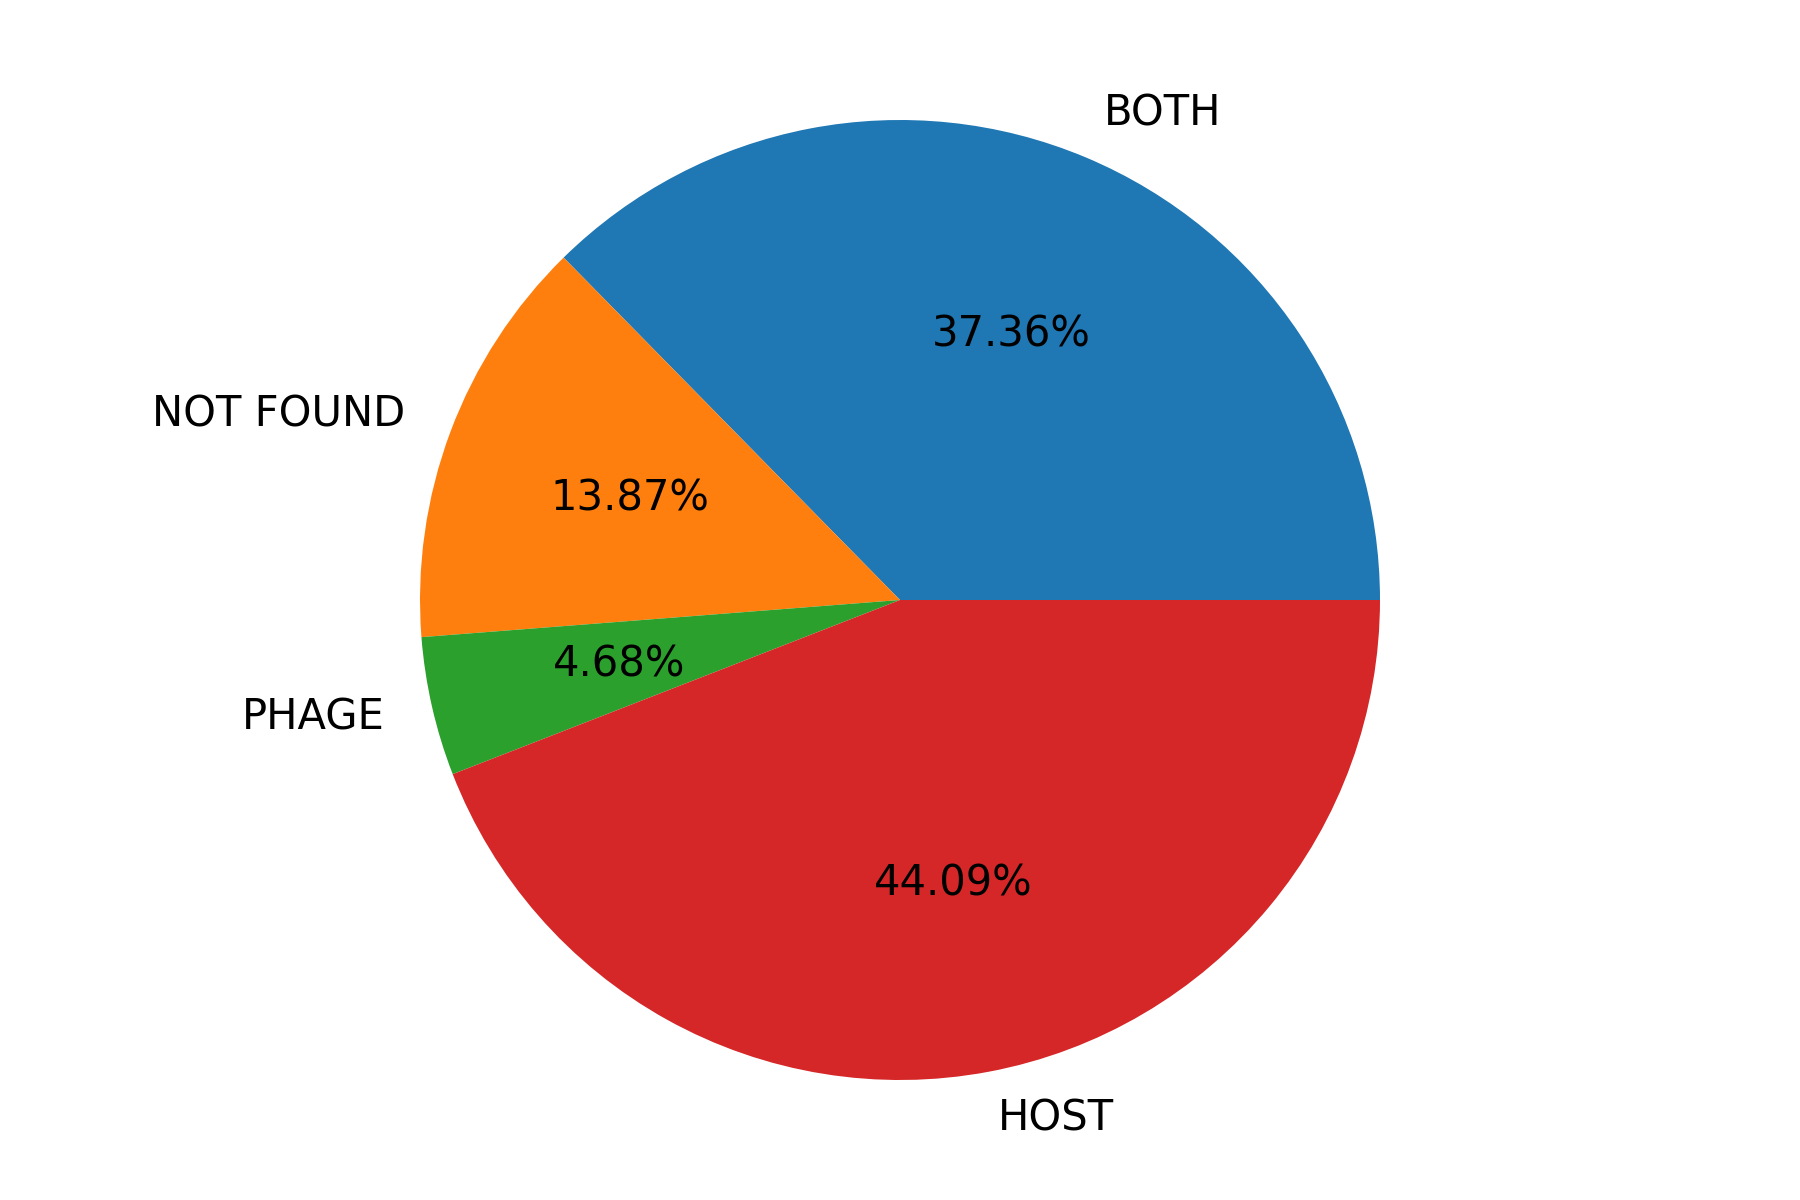
\includegraphics[width=\textwidth]{img/plot.png}
        \caption{Результат поиска мотивов по файлам без удаления -35 и -10 элементов. В процентном соотношении от 1946 
        мотивов.}
        \label{fig:skybox}
    \end{figure}
    
    \par{91 мотив был общим только у фагов, поражающих одну бактерию, но не был найден в самих бактериях, эти мотивы 
    были найдены в 53 исходных файлах. 858 мотивов было найдено внутри самих бактериальных промотрных областях, но они 
    не были найдены у фагов, поражающих эти бактерии. Они были найдены в 329 исходных файлах. И, наконец, 727 мотивов 
    были общими для бактерий и некоторых фагов, которые их поражают, они были найдены в 195 исходных файлах.  Оставшиеся
    270 найденных мотивов обладают мистическим свойством - они не были найдены ни в каких промоторных областях в своих 
    файлах.}

\par{Также, мы знаем, что у бактерии и у хоста могут часто повторяются -35 и -10 промоторные элементы. Нам они не
    были интересны. Мы нашли возможные последовательности для -35 и для -10 участков \cite{-35,-35-10,-35-10wiki} и 
    удалили их из нашего датасета с помощью регулярных выражений \cite{re}. В оставшейся таблице было 1344 мотива из 362
    исходных файлов. Из 
    них:} 
    
    \begin{itemize}
        \item 63 мотива были общими только среди фагов в 39 файлах.
        \item 624 мотива были найдены только среди областей бактериальных промоторов в 261 файле.
        \item 533 мотива были общими у хозяев и их фагов в 153 файлах.
        \item Также осталось 124 мистических мотива, которые не принадлежали ни фагам, ни бактериям в 104 файлах. 
    \end{itemize}
    
    \begin{figure}[h]
        \centering
        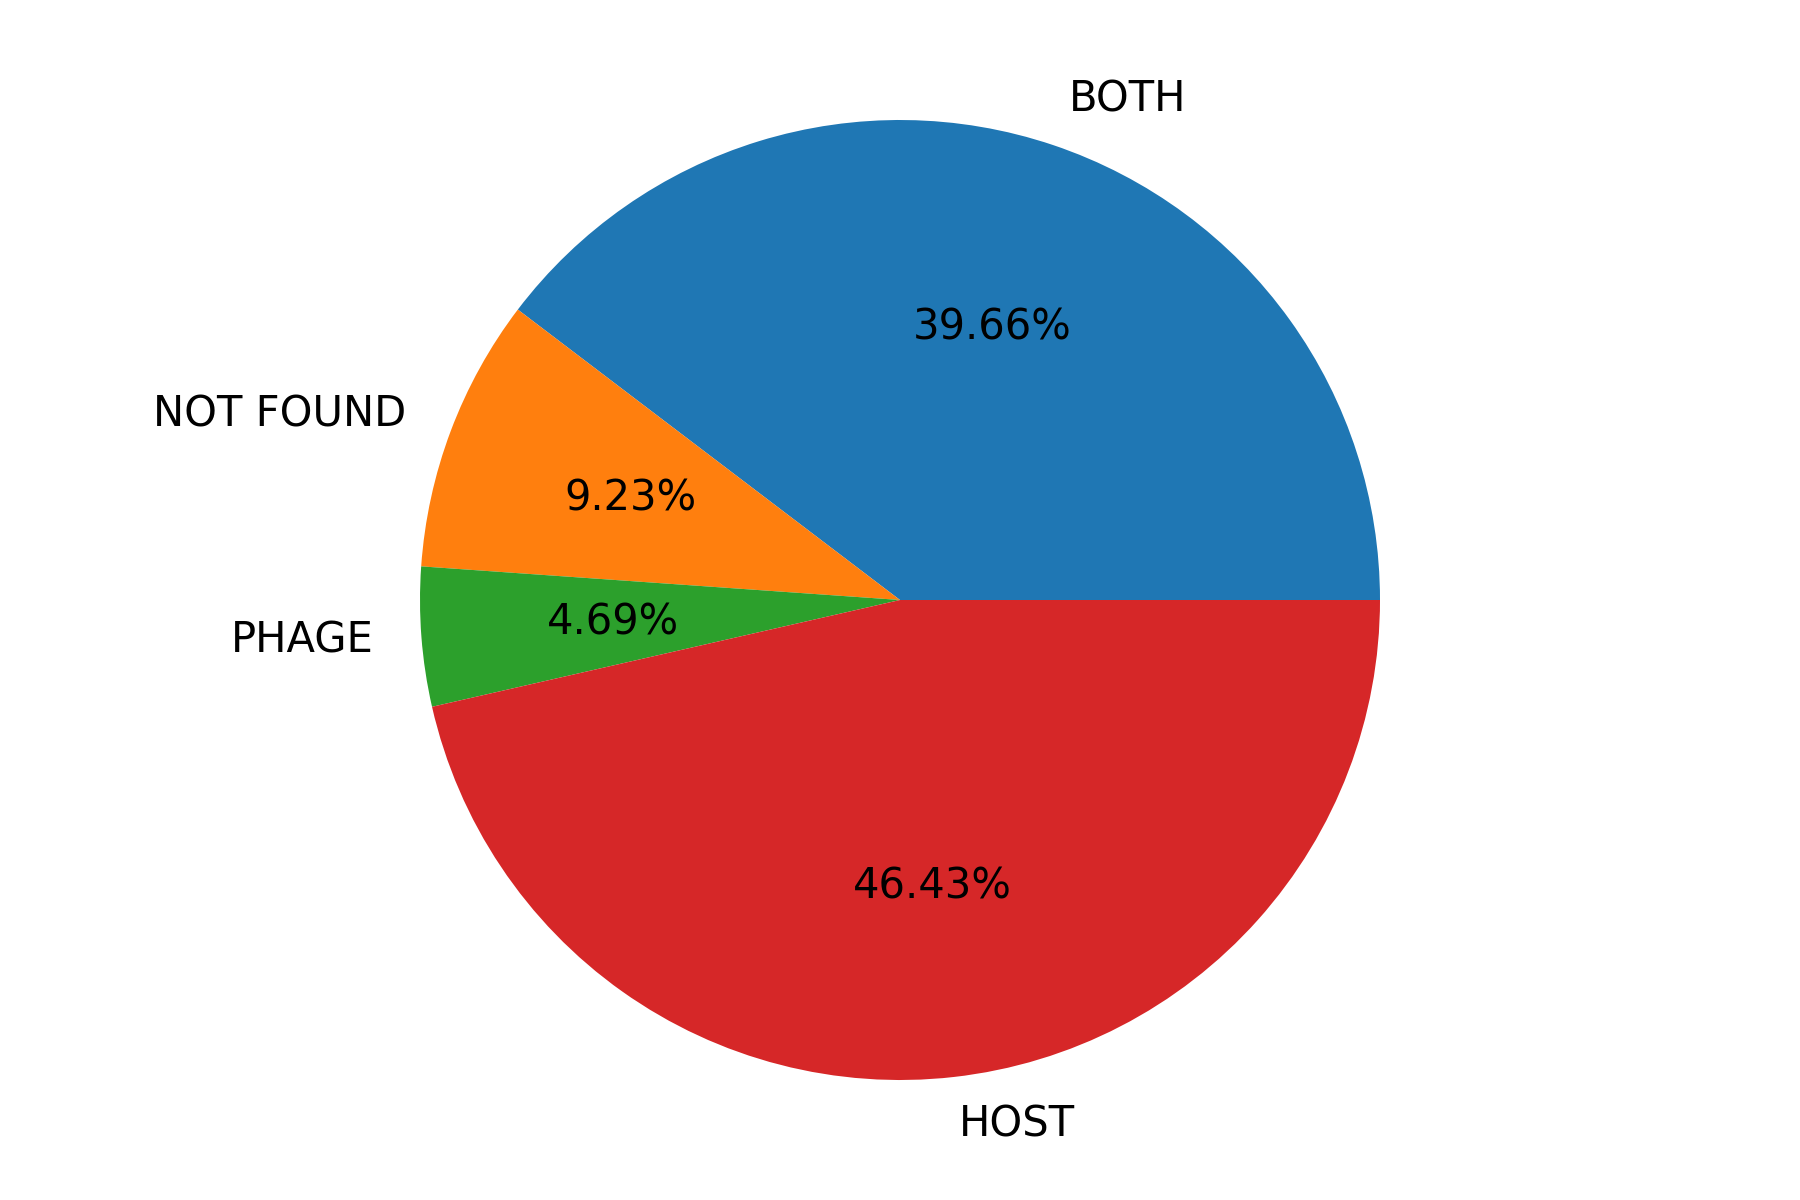
\includegraphics[width=\textwidth]{img/plot_.png}
        \caption{Результат поиска мотивов по файлам после удаления -35 и -10 элементов. В процентном соотношении от 1344 мотивов.}
        \label{fig:skybox}
    \end{figure}
    
    
    \par{Нам было интересно положение мотивов относительно начала транскрипции. Как уже было сказано, мы выделили 50 
    нуклеотидов - перед стартом транскрипции. Опять же, с помощью регулярных выражений, мы нашли положения мотивов в
    каждом 50-нуклеотидном регионе, в котором он встречается. Для каждого мотива мы посчитали среднее значение для его
    левого конца относительно начала транскрипции, для его правого конца и среднеквадратичную ошибку для обоих
    концов. Всё это зафиксировали в таблице результатов. Эта таблица получилось слишком большой, даже чтобы включать её в приложение. Она доступна по ссылке:
    \url{https://raw.githubusercontent.com/poolsar42/BachelorThesis/main/results.tsv}}

    \begin{figure}[h]
        \centering
        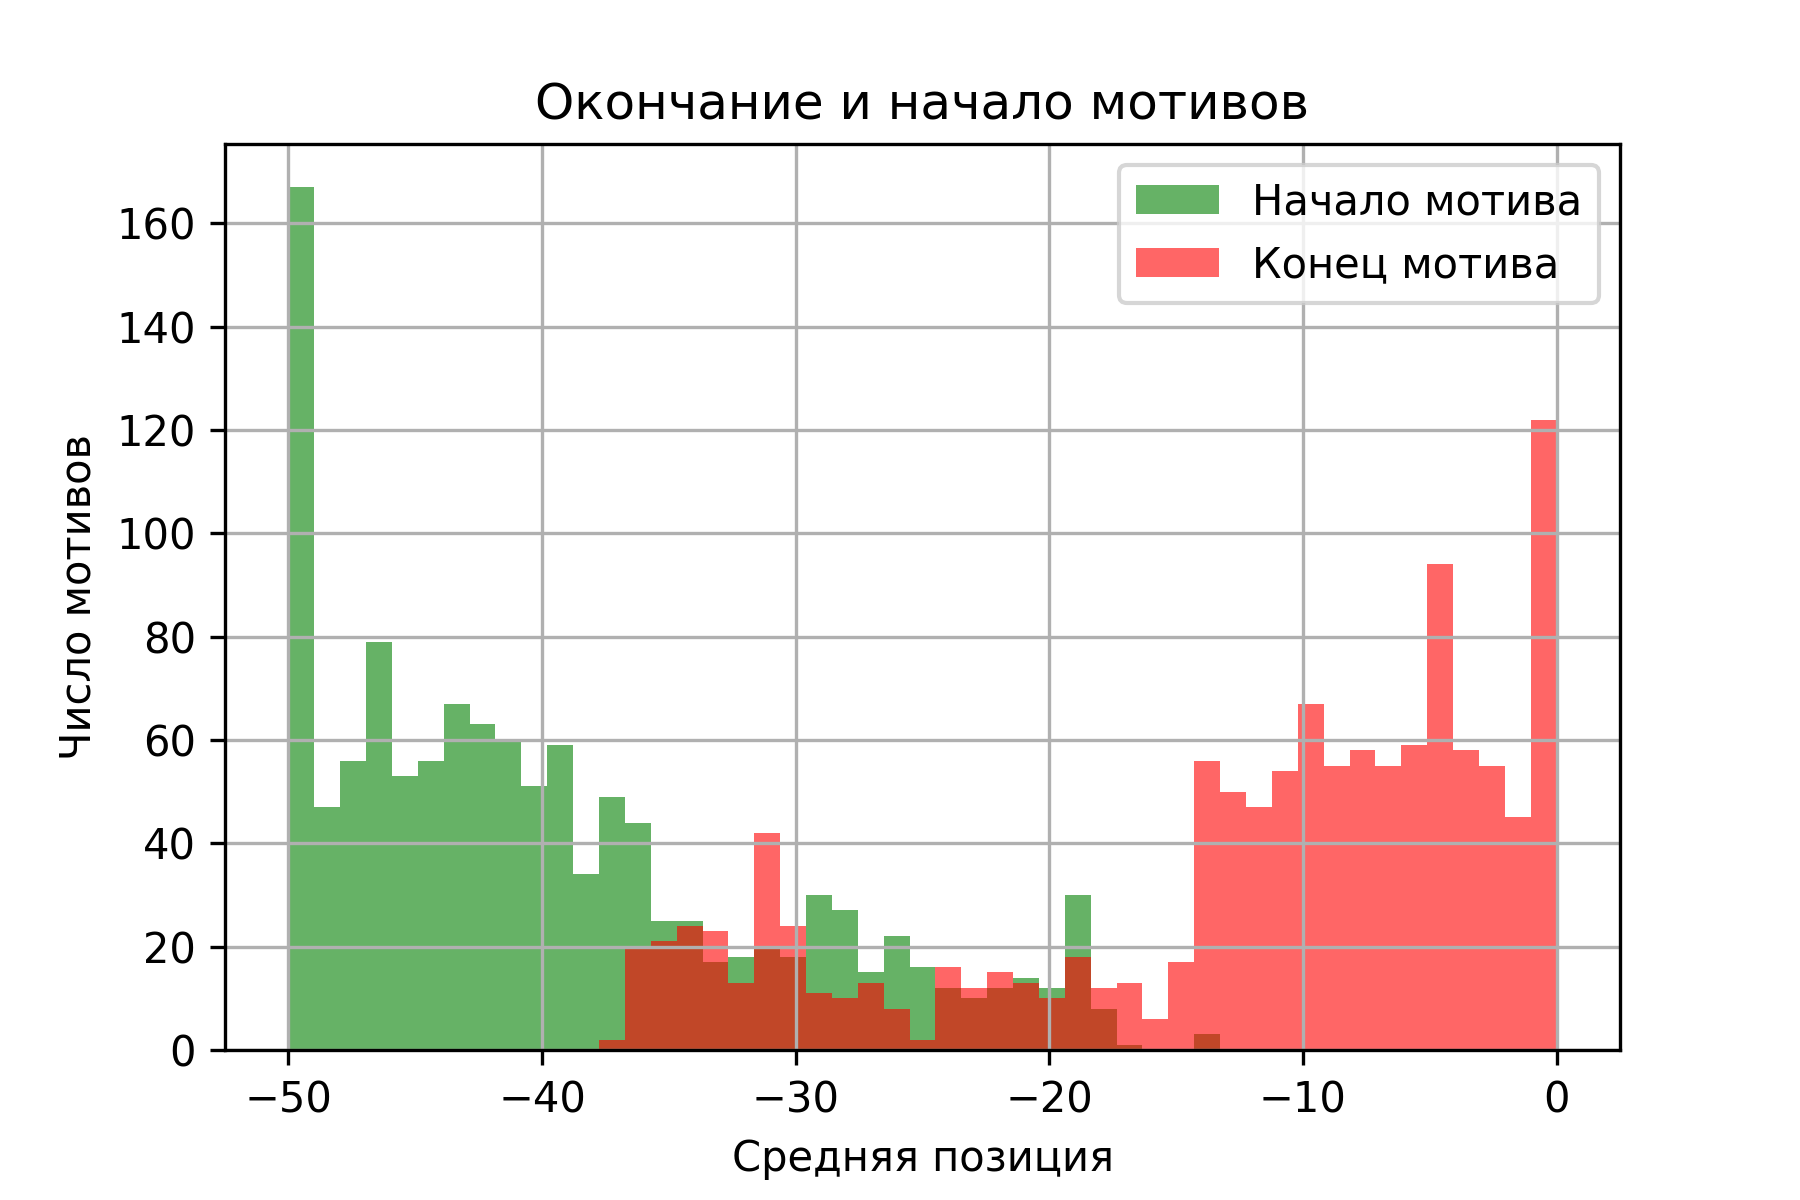
\includegraphics[width=\textwidth]{img/_plot_.png}
        \caption{Усреднённые для каждого мотива позиции его начала(зелёная гистограмма) и конца(красная).}
        \label{fig:skybox}
    \end{figure}
    
    \par{Также, как я уже написал выше, мы удивлись, когда обнаружили, что некоторые мотивы не были найдены ни в каком 
    из представленных вышестоящих регуляторных регионах. Также во многих мотивах 
    можно заметить большое количество букв W, N, Y и ещё некоторых, которые не входят в состав привычных нам A,T,G и C 
    для нуклеотидов. Дело в том, что на одном месте в мотиве в разных последовательностях могут стоять разные 
    нуклеотиды. И для таких двойственных мест MEME-Suite использует специальный алфавит, в котором одна буква заменяет 
    все возможные основания на данной позиции \cite{memealphabet}. }
    
    \par{Но когда мы начали анализировать эти последовательности, мы заметили, что некоторые регулярные выражения и 
    двойственные буквы, которые должны им соответствовать, не совпадают с теми, которые даны в алфавите 
    \cite{memealphabet}.}
    
    \par{ Минимальная ширина искомых мотивов была 10 нуклеотидов. Ширина нескольких известных 
    мотивов (-35, -10 etc.) колеблется в районе от 6 до 10 нуклеотидов. К тому же, межгенного расстояния в 
    50 нуклеотидов не всегда достаточно для поиска общих мотивов. Учитывая это, в 42\% случаях общие мотивы между фагами
    их хозяевами были найдены. В 54\% случаях общие мотивы были обнаружены только между фагами. Мы считаем эти первичные
    для данной задачи результаты вполне обнадёживающими. Процентные соотношения здесь не относительно общего числа 
    мотивов, а относительно общего числа файлов (видов бактерий).}
    
    \begin{center}
        \item \subsubsection{Корреляционный анализ}
    \end{center}

    \par{Нам также стало интересно, коррелируют ли как-то между собой мотивы бактериофагов, которые атакуют одну 
    бактерию, а также есть ли корреляция между мотивами бакториофагов из одной таксономической категории. Для начала мы 
    хотели посчитать корреляцию Пирсона между PFM этих мотивов. Но PFM - двумерный массив, мы не обнаружили в известных 
    библиотеках Python подходящей функции для подсчётка корреляции между 2D-массивами. Мы написали собственный скрипт 
    для предварительного подсчёта такой корреляции $preliminary_correlation.py$, используя трюки отсюда 
    \cite{stackoverflow}. Для кажого файла с мотивами была посчитана такого рода корреляция. На данном этапе результатры
    трудно интерпретировать. Опять же, приложу в качестве примера корреляционную матрицу для мотивов из одного файла. 
    Первый аргумент в каждой позиции этой матрицы - подсчитанный коэффициент корреляции Пирсона. Можно лишь заметить, 
    что везде наблюдается положительная корреляция, где-то в большей степени, а где-то в меньшей. Это указывает на то, 
    что действительно между мотивами фагов, атакующих одну бактерию есть что-то общее. Таблица доступна по ссылке: 
    \url{https://github.com/poolsar42/BachelorThesis/blob/main/MEME_0_1115_motif.tsv}}
    
    \newpage
    \begin{center}
    \item  \section{Выводы}
    \end{center}
    
    \begin{itemize}
        \item Наличие общих мотивов в регуляторных элементах бактериофагов и бактерий позволяет определить степень их 
        взаимоотношений.
        \item Наличие общих мотивов в регуляторных элементах между различными бактериофагами позволяет определить 
        степень родства этих бактериофагов.
    \end{itemize}
    
\newpage
\begin{thebibliography}{9}
    \addcontentsline{toc}{section}{\refname}
    \bibitem{hinton1} {Stitt B, Hinton DM: Regulation of middle-mode transcription.In Molecular biology  of  
    bacteriophage  T4.Edited by: Karam JD, Drake J, Kreuzer KN, Mosig G, Hall D, Eiserling F, Black L, Spicer E, Kutter 
    E, Carlson K, Miller ES.Washington, D.C.: American Society for Microbiology; 1994:142-160}
    \bibitem{hinton2} {Brody E, Rabussay D, Hall D:Regulation of transcription of prereplicative genes. In Bacteriophage
    T4.Edited by: Mathews CK, Kutter EM, Mosig G,Berget PB. Washington, D. C.: American Society for 
    Microbiology;1983:174-183}
    \bibitem{hinton3} Hinton, D.M. Transcriptional control in the prereplicative phase of T4 development. Virol J 7, 289
    (2010). https://doi.org/10.1186/1743-422X-7-289
    \bibitem{hinton4} Miller ES, Kutter E, Mosig G, Arisaka F, Kunisawa T, Ruger W: BacteriophageT4 genome. Microbiol  
    Mol  Biol  Rev2003,67:86-156
    \bibitem{hinton5} Wilkens K, Ruger W: Transcription from early promoters. In Molecular Biology  of  Bacteriophage  
    T4.Edited by: Karam JD, Drake JW, Kreuzer KN,Mosig G, Hall DH, Eiserling FA, Black LW, Spicer EK, Kutter E, Carlson 
    K,Miller ES. Washington, D. C.: American Society for Microbiology;1994:132-141.
    \bibitem{hinton6} Weisberg R, Hinton DM, Adhya S: Transcriptional Regulation in Bacteriophage. In Encyclopedia  of  
    Virology.3 edition. Edited by: Mahy BWJ,van Regenmortel MHV. Oxford: Elsevier; 2008:174-186, 174-186.
    \bibitem{virus-host} \url{https://www.genome.jp/virushostdb/}
    \bibitem{biopython} \url{https://biopython.org/}
    \bibitem{python} \url{https://docs.python.org/3/}
    \bibitem{jupyter} \url{https://jupyter.org/}
    \bibitem{github} \url{https://github.com/poolsar42/phages-and-hosts}
    \bibitem{entrez} \url{https://www.ncbi.nlm.nih.gov/books/NBK25501/}
    \bibitem{hinton} Hinton D.M. Transcriptional control in the prereplicative phase of T4 development // Virology
    journal. 2010. V. 7. P. 289. https://doi.org/10.1186/1743-422X-7-289
    \bibitem{puxty-evanx} Puxty, R.J., Evans, D.J., Millard, A.D. et al. Energy limitation of cyanophage development:
    implications for marine carbon cycling // ISME J. 2018, 12, 1273–1286. https://doi.org/10.1038/s41396-017-0043-3
    \bibitem{lomsad} Lomsadze, A., Gemayel, K., Tang, S., and Borodovsky, M. Modeling leaderless transcription and
    atypical genes results in more accurate gene prediction in prokaryotes // Genome research,  2018. 28(7), 1079–1089.
    https://doi.org/10.1101/gr.230615.117
    \bibitem{bailey} Bailey, T.L., Johnson, J., Grant, C.E., and Noble, W.S. The MEME Suite // Nucleic acids research,
    2015, 43(W1), W39–W49. https://doi.org/10.1093/nar/gkv416
    \bibitem{memeres} \url{https://kodomo.fbb.msu.ru/~partyhard/term4/pr9/meme_out_oops/meme.html#pssm1}
    \bibitem{-35} Promotors Addgene https://www.addgene.org/mol-bio-reference/promoters/
    \bibitem{-35-10} Chang-Hui Shen // Gene Expression: Transcription of the Genetic Code // Diagnostic Molecular 
    Biology, 2019 https://doi.org/10.1016/B978-0-12-802823-0.00003-1
    \bibitem{-35-10wiki} \url{https://en.wikipedia.org/wiki/Promoter_(genetics)#Bacterial}
    \bibitem{re} \url{https://docs.python.org/3/library/re.html#module-re}
    \bibitem{stackoverflow} \url{https://stackoverflow.com/questions/30143417/computing-the-correlation-coefficient-betw
    een-two-multi-dimensional-arrays}
    \bibitem{memealphabet} \url{https://meme-suite.org/meme/doc/alphabet-format.html#standard_DNA}
    \bibitem{meme} Bailey TL, Elkan C. Fitting a mixture model by expectation maximization to discover motifs in 
    biopolymers. Proc Int Conf Intell Syst Mol Biol. 1994;2:28-36. PMID: 7584402
    \bibitem{phagewikieng} \url{https://en.wikipedia.org/wiki/Bacteriophage}
    \bibitem{phageapps} Monk, A., Rees, C., Barrow, P., Hagens, S. and Harper, D. (2010), Bacteriophage applications: 
    where are we now? Letters in Applied Microbiology, 51: 363-369. https://doi.org/10.1111/j.1472-765X.2010.02916.x
    \bibitem{phagetreat} David R. Harper, Benjamin H Burrowes, Elizabeth M. Kutter (15 August 2014) Bacteriophage: 
    Therapeutic Uses, Letters in Applied Microbiology.  https://doi.org/10.1002/9780470015902.a0020000.pub2
    \bibitem{advdisphage} \url{https://sitn.hms.harvard.edu/flash/2018/bacteriophage-solution-antibiotics-problem/}
    \bibitem{17} Paget MS, Helmann JD: The sigma70 family of sigma factors. Genome Biol 2003, 4: 203. 
    10.1186/gb-2003-4-1-203
    \bibitem{20} Hook-Barnard IG, Hinton DM: Transcription Initiation by Mix and Match Elements: Flexibility for 
    Polymerase Binding to Bacterial Promoters. Gene Regulation and Systems Biology 2007. 
    http://la-press.com/article.php?article\_id=481:275-293
    \bibitem{4} Miller ES, Kutter E, Mosig G, Arisaka F, Kunisawa T, Ruger W: Bacteriophage T4 genome. Microbiol Mol 
    Biol Rev 2003, 67: 86-156. 10.1128/MMBR.67.1.86-156.2003
    \bibitem{91} Stoskiene G, Truncaite L, Zajanckauskaite A, Nivinskas R: Middle promoters constitute the most abundant
    and diverse class of promoters in bacteriophage T4. Mol Microbiol 2007, 64: 421-434. 
    10.1111/j.1365-2958.2007.05659.x
    \bibitem{39} Wilkens K, Ruger W: Characterization of bacteriophage T4 early promoters in vivo with a new promoter 
    probe vector. Plasmid 1996, 35: 108-120. 10.1006/plas.1996.0013
    \bibitem{3_} Zwirglmaier K, Jardillier L, Ostrowski M, Mazard S, Garczarek L, Vaulot D, et al. Global phylogeography
    of marine Synechococcus and Prochlorococcus reveals a distinct partitioning of lineages among oceanic biomes.
    Environ Microbiol. 2008;10:147–161.
    \bibitem{4_} Bouman HA, Ulloa O, Scanlan DJ, Zwirglmaier K, Li WKW, Platt T, et al. Oceanographic basis of the 
    global surface distribution of Prochlorococcus ecotypes. Science. 2006;312:918–921.
    \bibitem{5_} Scanlan DJ, Ostrowski M, Mazard S, Dufresne A, Garczarek L, Hess WR, et al. Ecological genomics of 
    marine picocyanobacteria. Microbiol Mol Biol Rev. 2009;73:249–299.
    \bibitem{6_} Biller SJ, Berube PM, Lindell D, Chisholm SW. Prochlorococcus: the structure and function of collective
    diversity. Nat Rev Microbiol. 2015;13:13–27.
    \bibitem{8_} Mann NH, Cook A, Millard AD, Bailey S, Clokie M. Bacterial photosynthesis genes in a virus. Nature. 
    2003;424:741–742.
    \bibitem{9_} Puxty RJ, Millard AD, Evans DJ, Scanlan DJ. Viruses inhibit CO2 fixation in the most abundant 
    phototrophs on Earth. Curr Biol. 2016;26:1585–1589.
    \bibitem{18_} Garczarek L, Dufresne A, Blot N, Cockshutt AM, Peyrat A, Campbell DA, et al. Function and evolution of
    the psbA gene family in marine Synechococcus: Synechococcus sp. WH7803 as a case study. ISME J. 2008;2:937–953.
    \bibitem{23_} Mulo P, Sakurai I, Aro EM. Strategies for psbA gene expression in cyanobacteria, green algae and 
    higher plants: From transcription to PSII repair. Biochim Biophys Acta Bioenerg. 2012;1817:247–257.
    \bibitem{24_} Imamura S, Yoshihara S, Nakano S, Shiozaki N, Yamada A, Tanaka K, et al. Purification, 
    characterization, and gene expression of all sigma factors of RNA polymerase in a cyanobacterium. J Mol Biol. 
    2003;325:857–872.
    \bibitem{25_} Imamura S, Asayama M, Shirai M. In vitro transcription analysis by reconstituted cyanobacterial RNA 
    polymerase: roles of group 1 and 2 sigma factors and a core subunit, RpoC2. Genes Cells. 2004;9:1175–1187.
    \bibitem{31_} Miller ES, Kutter E, Mosiq G, Arisaka F, Kunisawa T, Rüger W. Bacteriophage T4 genome. Microbiol Mol 
    Biol Rev. 2003;67:86–156.
    \bibitem{_1}   Altman, R, Brutlag, D, Karp, P, Lathrop, R, \& Searls, D. Proceedings: Second international 
    conference on intelligent systems for molecular biology. United States. 
    \bibitem{hyatt}  Hyatt D, Chen GL, Locascio PF, Land ML, Larimer FW, Hauser LJ. 2010. Prodigal: prokaryotic gene 
    recognition and translation initiation site identification. BMC Bioinformatics 11: 119
    \bibitem{bordov1}  Borodovsky M, McIninch JD, Koonin EV, Rudd KE, Medigue C, Danchin A. 1995. Detection of new genes
    in a bacterial genome using Markov models for three gene classes. Nucleic Acids Res 23: 3554–3562.
    \bibitem{fickett} Fickett JW, Tung CS. 1992. Assessment of protein coding measures. Nucleic Acids Res 20: 6441–6450
    \bibitem{bordov2} Borodovsky M, Sprizhitskii Y, Golovanov E, Aleksandrov A. 1986b. Statistical patterns in primary 
    structures of the functional regions of the genome of Escherichia coli. Computer recognition of coding regions. Mol 
    Biol 20
    
\end{thebibliography}

\end{document}
